\cleardoublepage
\chapter{Background and Related Work}
\label{cha:background}
The main contributions of this thesis revolve around the SimRa project (see section~\ref{subsec:simra}), which is a crowdsourcing/crowdsensing citizen science application, with the goal of improving cycling comfort and cycling safety.
In this chapter, we go through fundamental topics that are needed to better understand the nature of the SimRa project and thus, the contributions outlined in chapter~\ref{cha:contributions}.
For this, we first outline which factors mainly influence cycling comfort and give an overview of recent studies from that research area in section~\ref{sec:cycling_comfort_background}.
We then continue with cycling safety in section~\ref{sec:cycling_safety_background}, which is related to cycling comfort.
There, we also differentiate between bicycle safety and bicycle traffic safety.
In chapter~\ref{sec:crowdsourcing_crowdsensing_background}, we point out similarities and differences between crowdsourcing and crowdsensing, so that we can later, in section~\ref{subsec:simra}, better categorize the SimRa project between them.
Lastly, to complete this chapter, we take a brief look into the field of citizen science, namely what makes a project a citizen science project, which benefits and challenges it brings and how the related work makes use of it in chapter~\ref{sec:citizen_science_background}. 

\section{Cycling Comfort}
\label{sec:cycling_comfort_background}
Other edge-assisted data analysis work includes Mei et al.~\cite{mei2017ultraviolet}, who measure UV radiation based on smartphone cameras and crowdsensing,
Cao et al.~\cite{cao2015fast} who use motion sensors to detect strokes in patients falling to the ground, and
Pham et al.~\cite{pham2015a} implement a smart parking system by equipping parking spots with RFID chips to track their occupancy state.
There are also multiple publications on placing different components of an edge-to-cloud data processing pipeline in various use cases, e.g.,~\cite{lujic2021increasing,pfandzelter2021zero,hattab2019optimized}.


\section{Cycling Safety}
\label{sec:cycling_safety_background}
Other edge-assisted data analysis work includes Mei et al.~\cite{mei2017ultraviolet}, who measure UV radiation based on smartphone cameras and crowdsensing,
Cao et al.~\cite{cao2015fast} who use motion sensors to detect strokes in patients falling to the ground, and
Pham et al.~\cite{pham2015a} implement a smart parking system by equipping parking spots with RFID chips to track their occupancy state.
There are also multiple publications on placing different components of an edge-to-cloud data processing pipeline in various use cases, e.g.,~\cite{lujic2021increasing,pfandzelter2021zero,hattab2019optimized}.


\section{Crowdsourcing and Crowdsensing}
\label{sec:crowdsourcing_crowdsensing_background}
crowdsourcing and crowdsensing have emerged as successful approaches to solve tasks in a fast and cost-efficient way and gather big amounts of data in a short time respectively.

\subsection*{Crowdsourcing}
``Crowdsourcing'' is a combination of the words \textit{crowd} and \textit{outsourcing}.
\textit{Crowd} refers to an often larger group of individuals, to which a task is transferred to, whereas outsourcing refers to a practice where an entity does not fulfill a task in-house on it's own, but hires people from outside to solve a task for them.
Crowdsourcing comes in many shapes and forms and can be found in many different areas, from transportation, to financing, from social media to natural crisis relief, etc.
A very common form of crowdsourcing is the so called mobile crowdsourcing.
The difference is that in mobile crowdsourcing the the people fulfilling the task usually do not have to be stationary, but rather mobile, because the task at hand demands movement or being in a specific location to be fulfilled.
In the latter case, a smartphone or a hardware device containing some sort of sensors has to be used by the participants to fulfill the task.
For the remainder of this work, we will use the terms crowdsourcing and mobile crowdsourcing interchangeably.

Figure~\ref{fig:crowdsourcing} shows the key elements of crowdsourcing.
In the top layer, the application (e.g., a ride-hailing app) requests a task (e.g., a ride from location A to location B).
The data processing layer gets this task and determines who (e.g., which taxi drivers) this task should be allocated to.
Then, the crowd (e.g., the taxi driver, that got the task) completes the task.
After that, the result (e.g., the arrival of the customer at the destination) is sent to the data-processing layer again, where the results are processes and aggregated and the end result is sent to the application (e.g., invoice).

\begin{figure}[htbp]
  \centering
  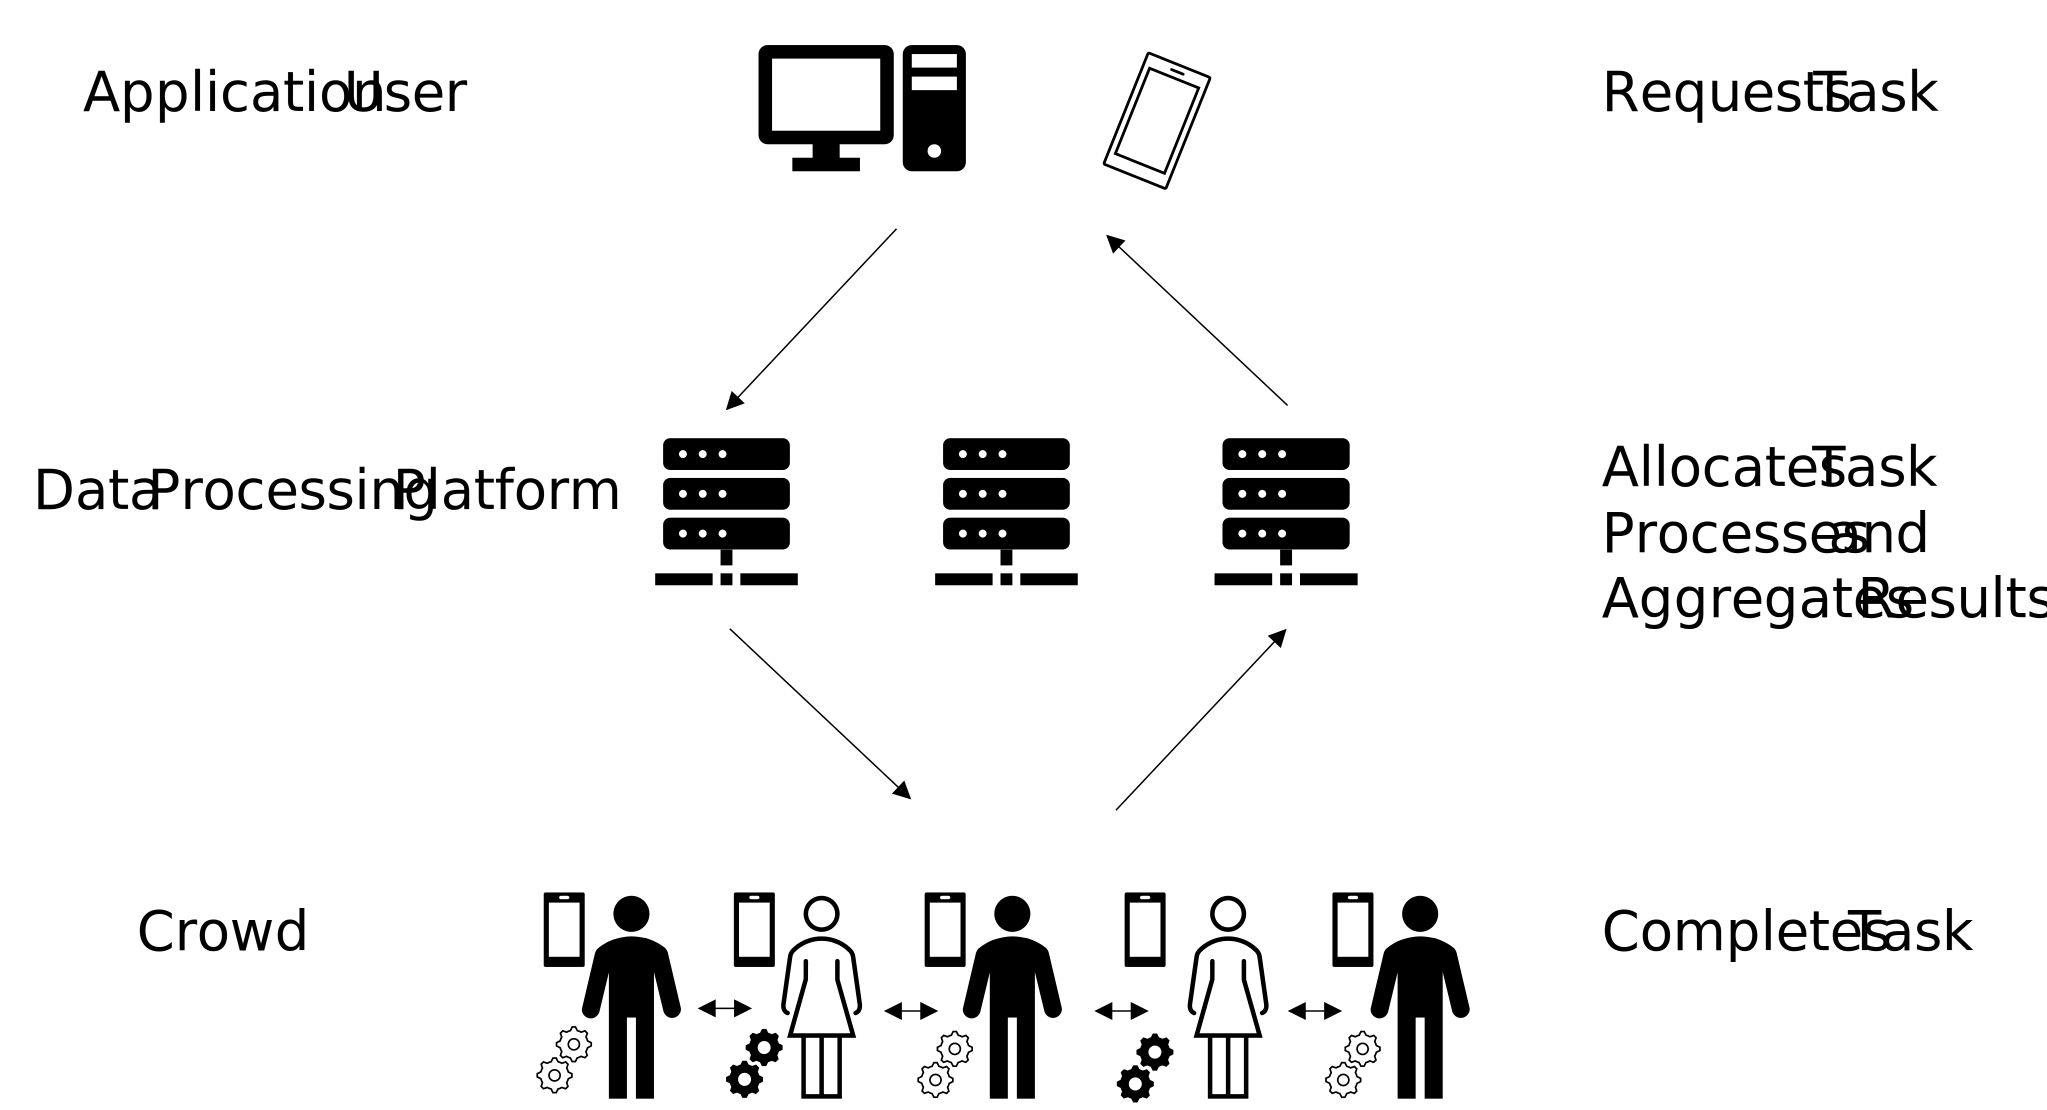
\includegraphics[width=0.8\textwidth]{fig/crowdsourcing.pdf}
  \caption{svg image}
\end{figure}
\label{fig:crowdsourcing}

There are different aspects that characterize a crowdsourcing application: \textit{degree of human involvement}, \textit{location relevance}, \textit{knowledge requirement}, \textit{participation incentive} and \textit{data flow}.

There are two types of \textit{degree of human involvement}: Opportunistic and Participatory.
The former describes that the participant is not actively operate the smartphone or device, while in the latter, the user has to give further input on the smartphone or device.
The \textit{degree of human involvement} is a continuum, where each crowdsourcing application can have different levels of human involvement.

\textit{Location relevance} indicates how important it is that the task has to be solved at a specific location.
With mobile crowdsourcing, a certain degree of \textit{location relevance} is naturally given, but there still can be different levels of \textit{location relevance}.
For instance, the task may need to be completely done at a specific locations, or only parts of it, such as taking a photo of a location but then editing the photo anywhere.
Similar to \textit{degree of human involvement}, here we also have a continuum, being between high location relevance and no location relevance.

\textit{Knowledge requirement} refers to the level of knowledge that the participant needs to fulfill a given task.
Some tasks may be very simple, where detailed knowledge is unnecessary, while other tasks may need some experts of a specific topic or an extensive training to be able to solve the task.
A high \textit{knowledge requirement} may make it necessary to distinctively allocate the task to such participants, where the \textit{knowledge requirements} are met.

The \textit{participation incentive} can vary from project to project and also from participant to participant.
There are basically two types of incentives: intrinsic and extrinsic.
A participant with an intrinsic incentive engages with a crowdsourcing project, because he/she can identify with the problem the project wants to solve or simply likes to to perform the task.
There can also be extrinsic motivations such as getting paid in cash or with coupons, or gaining social credits for it.
It is very much possible, that participants have both intrinsic \textit{and} extrinsic incentives to participate in a project.

The \textit{data flow} is a technical aspect of the crowdsourcing project.
Here, there are three distinctions: centralized, decentralized and hybrid.
When the data flows from the crowd directly to the processing platform, the project has a centralized data flow.
Contrary to that, when the data flow is decentralized, it means that some participants' devices collect the solved tasks in the crowd and then send it in aggregated form to the processing platfrom.
This may be beneficiary to decrease the load on the processing platform.
A hybrid form is also possible, where the processing platform gets bypassed and the data produced by the participants is also processed in the crowd to be sent to the application directly. 

\subsection*{Crowdsensing}
As in ``Crowdsourcing'' the crowd in ``Crowdsensing'' refers to a group of people, who voluntarily take over a task.
However, in crowd\textit{sensing}, the task at hand is mainly to gather data for the client, or in other words to function as a sensor.



\section{Citizen Science}
\label{sec:citizen_science_background}